\documentclass[journal,10pt,twocolumn]{article}
\usepackage{graphicx}
\usepackage[margin=0.5in]{geometry}
\usepackage{array}
\usepackage{amsmath}
\usepackage{booktabs}
\title{\textbf{Line Assignment}}
\author{Alavala Chinnapa Reddy}
\date{September 2022}

\begin{document}

\maketitle
\paragraph{\textit{Problem Statement} - The side AB of a parallelogram ABCD is produced to any point P. A line through A and parallel to CP meets CB produced at Q and then parallelogram PBQR is completed.Show that}
\begin{enumerate}
  \item \textbf{ar(ABCD) = ar(PBQR)}
\end{enumerate}

\begin{figure}[h]
\centering
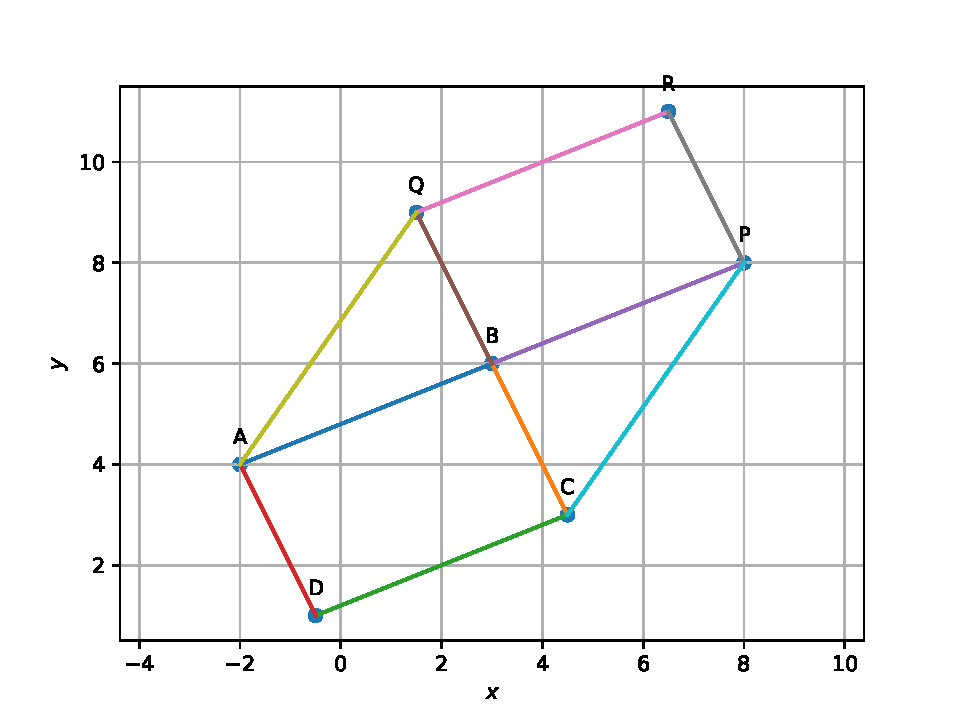
\includegraphics[width=1\columnwidth]{figs/l1.pdf}
\caption{parallelogram PBQR is produced using parallelogram ABCD}
\end{figure}

\section*{Solution}
\subsection*{METHOD 1}

Let 
\begin{equation}
\boldsymbol{B-A} = \boldsymbol{m}
\end{equation}
\begin{equation}
\boldsymbol{D-A} = \boldsymbol{n} 
\end{equation}
n written as two perpendicular components one along $\boldsymbol{m}$ and one perpendicular to $\boldsymbol{m}$
\begin{equation}
   \boldsymbol{n}=\boldsymbol{m} \parallel_A +\boldsymbol{m} \perp_A
\end{equation}
\begin{equation}
\boldsymbol{m} \parallel_A ={\frac{\boldsymbol{n}^T\boldsymbol{m}}{||\boldsymbol{m}||^2}}\boldsymbol{m}
\end{equation}
\begin{equation}
\boldsymbol{m} \perp_A =\boldsymbol{n} - \boldsymbol{m} \parallel_A
\end{equation}
\begin{equation}
\boldsymbol{m} \perp_A=\boldsymbol{n}-{\frac{\boldsymbol{n}^T\boldsymbol{m}}{||\boldsymbol{m}||^2}}\boldsymbol{m}
\end{equation}
\begin{equation}
||\boldsymbol{m} \perp_A||^2=||\boldsymbol{n}||^2-{\frac{{\boldsymbol{n}^2T\boldsymbol{m}}^2}{||\boldsymbol{m}||^2}}
\end{equation}
\begin{eqnarray}
    Area of parallelogram ABCD =\sqrt{{base}^2{height}^2}\\
    Area of parallelogram ABCD =\sqrt{{||\boldsymbol{m} \perp_A}||^2{||\boldsymbol{m}||^2}}\\
    Area of parallelogram ABCD =\sqrt{(||\boldsymbol{n}||^2-{\frac{{\boldsymbol{n}^2T\boldsymbol{m}}^2}{||\boldsymbol{m}||^2}})||\boldsymbol{m}||^2}
\end{eqnarray}
Let\\
Q lies on BC extended
\begin{eqnarray}
    \boldsymbol{P}=\boldsymbol{B}+x\boldsymbol{m}\\
    \boldsymbol{Q}=\boldsymbol{B}+k\boldsymbol{n}
\end{eqnarray}
Q line passes through A and parallel to CP
\begin{equation}
    \boldsymbol{Q}=\boldsymbol{A}+u\boldsymbol{o}
\end{equation}
where
\begin{equation}
	\boldsymbol{o}=\boldsymbol{P}-\boldsymbol{C}    
\end{equation}
equating 13 and 14
\begin{eqnarray}
	\boldsymbol{B}+k\boldsymbol{n}=\boldsymbol{A}+u\boldsymbol{o}\\
    B-A=u\boldsymbol{o}-k\boldsymbol{n}
    \end{eqnarray}
\begin{equation}
	\textbf{B-A}=
\begin{pmatrix}
    \boldsymbol{o} & -\boldsymbol{n}
\end{pmatrix}
\begin{pmatrix}
    u\\
    k
\end{pmatrix}
\end{equation}
\begin{equation}
\begin{pmatrix}
    u\\
    k
\end{pmatrix}
=
\begin{pmatrix}
    \boldsymbol{o} & -\boldsymbol{n}
\end{pmatrix}^{-1}
	\textbf{(B-A)}
\end{equation}
OR
\begin{equation}
k={e2}^T
\begin{pmatrix}
    \boldsymbol{o} & -\boldsymbol{n}
\end{pmatrix}^{-1}
	\textbf{(B-A)}
\end{equation}
for parallelogram \textbf{PQRS}, \\
Base =$||\boldsymbol{P}$-$\boldsymbol{B}||$
\begin{equation}
Base=x||\boldsymbol{m}||(from-eq12)
\end{equation}
To find height, write $\boldsymbol{Q}-\boldsymbol{B}$ as sum of two perpendicular components
\begin{equation}
    \boldsymbol{Q}-\boldsymbol{B}=k\boldsymbol{n}
\end{equation}
\begin{equation}
    \boldsymbol{Q}-\boldsymbol{B}=\boldsymbol{m} \parallel_P +\boldsymbol{m} \perp_P
\end{equation}
\begin{equation}
    \boldsymbol{m} \parallel_P=k{\frac{\boldsymbol{n}^T\boldsymbol{m}}{||\boldsymbol{m}||^2}}\boldsymbol{m}
\end{equation}
\begin{equation}
\boldsymbol{m} \perp_P=k(\boldsymbol{n}-{\frac{\boldsymbol{n}^T\boldsymbol{m}}{||\boldsymbol{m}||^2}}\boldsymbol{m})
\end{equation}
compare eq 6 and eq 24
\begin{equation}
\boldsymbol{m} \perp_P=k(\boldsymbol{m} \perp_A)
\end{equation}
From eq20
\begin{equation}
	Base\textbf{PB}=|\boldsymbol{P}-\boldsymbol{B}=x||\boldsymbol{m}||=x(||\boldsymbol{A}-\boldsymbol{B}||)=Base\textbf{AB}
\end{equation}
From eq25 and eq26\\
Area of parallelogram=$|\boldsymbol{m}\perp_P|$(Base\textbf{PB})\\
=k($|\boldsymbol{m}\perp_A|$)x(Base\textbf{AB})
\begin{equation}
	=kx(area(\textbf{ABCD}))
\end{equation}
Let\\
Point B be
$\begin{pmatrix}
    0&0
\end{pmatrix}$
, A be 
$\begin{pmatrix}
    i \\
    0
\end{pmatrix}$
and D=
$\begin{pmatrix}
    j\\
    k
\end{pmatrix}$.
The figure can be relocated to other origin and rotated by transformation Py+C without any changes.So,results valid with assume points A,B and D is valid.
\begin{equation}
	\boldsymbol{o}=\boldsymbol{P}-\boldsymbol{C}=\boldsymbol{B}+x\textbf{(B-A)-((B-A)+(D-A)+A)}
\end{equation}
\begin{equation}
    \boldsymbol{o}=x\boldsymbol{B}+(1-x)\boldsymbol{A}-\boldsymbol{D}
\end{equation}
\begin{equation}
    \boldsymbol{o}=
    \begin{pmatrix}
        (1-x)i-j\\
        -k
    \end{pmatrix}
\end{equation}
\begin{equation}
    -\boldsymbol{n}=-(\boldsymbol{o}-\boldsymbol{A})=
    \begin{pmatrix}
        i-j\\
        -k
    \end{pmatrix}
\end{equation}
\begin{equation}
    (\boldsymbol{o}-\boldsymbol{A})=
    \begin{pmatrix}
        (1-x)i-j & i-j \\
        -k       & -k
    \end{pmatrix}
\end{equation}
\begin{equation}
     (\boldsymbol{o}-\boldsymbol{A})^-1=
     \begin{pmatrix}
         -k & j-i\\
         k  & (1-x)i-j
     \end{pmatrix}
     (\frac{1}{det((\boldsymbol{o}-\boldsymbol{n}))})
\end{equation}
$det(\boldsymbol{o}-\boldsymbol{n})=(x-1)ki+kj-kj+ki$\\
$det(\boldsymbol{o}-\boldsymbol{n}=xki$\\
substuting eq33 in eq19
\begin{eqnarray}
    k=(\frac{1}{xki})
    \begin{pmatrix}
        0 & 1
    \end{pmatrix}
    \begin{pmatrix}
        -k & j-i\\
        k & (1-x)i-j
    \end{pmatrix}
    \begin{pmatrix}
        -i\\
        0
    \end{pmatrix}\\
    k=(\frac{1}{xki})
    \begin{pmatrix}
        0 &1
    \end{pmatrix}
    \begin{pmatrix}
        ki\\
        -ki
    \end{pmatrix}\\
    k=(\frac{1}{xki})(-ki)=\frac{-1}{x}
\end{eqnarray}
sub eq36 in eq27\\
area(\textbf{PBQR})=$(\frac{-1}{x})(x)aera(\textbf{ABCD})$\\
Finally\\
      $|aera(\textbf{PBQR})|=|aera(\textbf{ABCD})|$
      \subsection*{METHOD 2}
GIVEN \textbf{ABCB} is parallelogram\\
     \textbf{AB}$\parallel$\textbf{CB} and \textbf{BC}$\parallel$\textbf{DA}\\
     P is extension of AB \\
     Q is extension of CB \\
     \textbf{PBQR} parrallelogram is produced \\
     \textbf{CP}$\parallel$\textbf{AQ}\\
     From the above \\
     We Know
     \begin{eqnarray}
         \textbf{Q-B}=\lambda_1(\textbf{D-A})\\
     \textbf{P-B}=\lambda_2(\textbf{C-D})\\
     \textbf{B-A}=\textbf{A-D}\\
     \textbf{B-C}=\textbf{A-D}\\
     \textbf{R-P}=\textbf{Q-B}\\
     \textbf{R-Q}=\textbf{P-B}\\
      \textbf{Q-A}=\lambda(\textbf{P-C})
     \end{eqnarray}
     Where $\lambda=(\lambda_1)*(\lambda_2)$\\
     using A,B,C,D,P,Q,R Position Vectors\\
     We find\\
     From eq37,$\lambda_1=1$\\
     From eq38,$\lambda_2=1$\\
     Finally
     \begin{equation}
         \lambda=(\lambda_1)*(\lambda_2)=1
     \end{equation}
We Know \\
 Area of parallelogram \textbf{ABCD}=$\textbf{AB} \times \textbf{AD}$\\
 $\angle(AB,AD)=\theta$
 \begin{equation}
     \theta=\arccos(\frac{\textbf{AB}\cdot\textbf{AD}}{|AB|*|AD|})
 \end{equation}
 Using Position Vectors\\
$\theta=17.64$\\
 Area of parallelogram \textbf{ABCD}=$|\textbf{AB}||\textbf{AD}|\sin{\theta}$\\
 using Position Vectors
\begin{equation}
     Area of parallelogram \textbf{ABCD}=5.47 \textbf{square units}
\end{equation}
Area of parallelogram \textbf{PBQR}=$\textbf{QB} \times \textbf{BP}$\\
 $\angle(QB,BP)=\alpha$
 \begin{equation}
     \alpha=\arccos(\frac{\textbf{QB}\cdot\textbf{BP}}{|QB|*|BP|})
 \end{equation}
 Using Position Vectors\\
$\alpha=17.64$\\
 Area of parallelogram \textbf{PBQR}=$|\textbf{QB}||\textbf{BP}|\sin{\alpha}$\\
 using Position Vectors
\begin{equation}
     Area of parallelogram \textbf{PBQR}=5.47 \textbf{square units}
\end{equation}
From eq44,eq46 and eq48\\
Finally\\
Area of parallelogram \textbf{ABCD}=Area of parallelogram \textbf{PBQR}
\section*{Construction}
The input parameters are the values i,j,k,x.\\
{
\setlength\extrarowheight{2pt}
\begin{tabular}{|c|c|c|}
  \hline
  \textbf{Symbol}&\textbf{Value}&\textbf{Description}\\
  \hline
  i&-2&\\
  \hline
  j&-0.5&\\
  \hline
  k&1&\\
  \hline
  x&-1&\\
  \hline
	\textbf{A}&
	$\begin{pmatrix}
		i\\
		4
	 \end{pmatrix}$
  &Position Vector A\\
  \hline
	\textbf{B}&
	$\begin{pmatrix}
		3\\
		6
	\end{pmatrix}$
	&Position Vector B\\
  \hline
	\textbf{D}&$
   \begin{pmatrix}
		j\\
		k
    \end{pmatrix}$
	& Position Vector D\\
  \hline
	\textbf{C}&D+B-A&Position Vector C\\
  \hline
	\textbf{m}&B-C&Diretion Vector of AB\\
  \hline
	\textbf{n}&D-A&Diretion Vector of DA\\
  \hline
	\textbf{P}&B-x*m&Position Vector P\\
  \hline
	\textbf{Q}&B+x*n&Position Vector Q\\
  \hline
	\textbf{R}&P+Q-B&Position Vector R\\
  \hline
\end{tabular}
}
\end{document}
